% Metódy inžinierskej práce

\documentclass[10pt,a4paper]{article}

%\usepackage[T1]{fontenc}
\usepackage[utf8]{inputenc}
\usepackage{graphicx}
\usepackage{url} % príkaz \url na formátovanie URL
\usepackage{hyperref} % odkazy v texte budú aktívne (pri niektorých triedach dokumentov spôsobuje posun textu)
\usepackage{array}
\usepackage{cite}
\usepackage{enumitem}
\usepackage{caption} 
%\usepackage{times}

\pagestyle{headings}

\title{Improvement of indexing and semantic search methods \thanks{Semestrálny projekt v predmete Metódy inžinierskej práce, ak. rok 2023/24, vedenie: Bohdan Koval}} % meno a priezvisko vyučujúceho na cvičeniach

\author{Bohdan Koval\\[2pt]
	{\small Slovenská technická univerzita v Bratislave}\\
	{\small Fakulta informatiky a informačných technológií}\\
	{\small \texttt{xkoval@stuba.sk}}
	}

\date{\small 30. october 2023} % upravte



\begin{document}

\maketitle

\begin{abstract}
\ldots
\end{abstract}



\section{Intodruction}

Nowadays we constantly use web to search for information. And it always answers on our questions quickly and correct. But how does it work? How does the web understand our request and choose the best websites? In this article I will try to explain how it works and give some ideas how it can be improved.

Article will include several topics:
\begin{enumerate}
  \item How do web engines search for the answers on queries?
  \item What is indexing method?
  \item How indexing method works?
  \item What is semantic search method?
  \item How can these methods be improved?
\end{enumerate}



\section{Understanding Indexing} \label{nejaka}
 Indexing is the process of creating an index, which is a structured data structure that maps (words, phrases, or other elements) to the locations or records where they appear in web pages, or any other source of information.

 Long story short it's a process of organizing the information before a search to enable faster answers on queries.
 
Searching for keywords through whole web page would be a very long task. Because of it search engines use some methods to optimize this process. But before we should go through process that operate with text and make it easier to analyze.



\subsection{Processes}

The most logic process is "Tokenization".

Tokenization is essentially splitting a phrase, sentence, paragraph, or an entire text document into smaller units, such as individual words or terms. Each of these smaller units are called tokens.

So now let's try it on an example.

Engine will have a query : 
\textbf{It's not a bug. It's an undocumented feature.}

That how it will look after Tokenization:

\begin{center}
\begin{itemize}[label={}]
    \centering
    \item \texttt{["It's"]}
    \item \texttt{["not"]}
    \item \texttt{["a"]}
    \item \texttt{["bug"]}
    \item \texttt{["It's"]}
    \item \texttt{["an"]}
    \item \texttt{["undocumented"]}
    \item \texttt{["feature"]}
\end{itemize}
\end{center}

It is the easiest example - Tokenization by words. There are much more types but the main task was to understand the idea.

\hrulefill

Stop Words Removal it's another quite easy and logic process. That remove words like "and", "is", "a", "the". This process is just created to make text shorter and as a result easier to analyze.

\hrulefill

Stemming and Lemmatization it's the process that reduce the word to it's root. For example running -> run; better -> good. This process ensure that different inflections of the word will be treated in the same word.

\hrulefill

Normalization is the last proces in my list that just convert all text to lower case.

\hrulefill


\subsection{Indexing methods}
\subsubsection{Inverted Index definition}
Inverted Index method is the most popular method nowdays. So I will talk about it the first.

Inverted Index is a data structure that organized by terms(words), and each term points to a list of web pages that contain it. It can also be interpreted as hash-map, with words on the place of the key.


\begin{figure}
  \centering
  \captionsetup{labelformat=empty}  % Removes the label (e.g., "Figure")
  \caption{Types of inverted indexes.}
  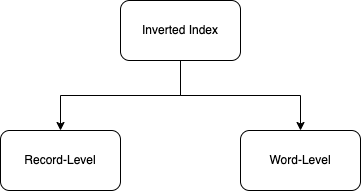
\includegraphics[width=0.6\textwidth]{for_mip.drawio.png}  % Replace 'example-image' with your image file name and specify the width
  
  \begin{enumerate}[label=\textbullet]
      \item Record-Level Inverted Index: This type of index maintains a collection of document references for each individual word.
      \item Word-Level Inverted Index additionally contains the positions of each word within a document.
  \end{enumerate}
\end{figure}

\hrulefill

\subsubsection{Steps to Build an Inverted Index}

It's comfortable in this case to use "Tokenization", "Normalization" and "Streaming". And as data structure hash-map or basic map. 

For each (term)word check if it already exist in the "list". If not add, else add the name(name and location in the web-page) of the web-page(document) to key equal to the (term)word.


\subsubsection{Example of Inverted Index}
\begin{minipage}{0.7\textwidth}
  \textbf{Sentence 1}: This is my cat, he is black.

  \textbf{Sentence 2}: Is this your black cup.
\end{minipage}

\begin{figure}[h]
  \centering
  \captionsetup{labelformat=empty}
  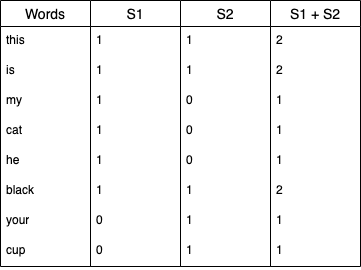
\includegraphics[width=0.6\textwidth]{example.png}  % Replace 'example.png' with your image file name and specify the width
  \caption{\textbf{Record-Level}}
\end{figure}

\subsubsection{Forward Index definition}

Forward Index Method: The Forward Index method shares a similar underlying structure with the Inverted Index, often implemented as a hash-map, but it uses a distinct approach. In the Inverted Index, the key is typically a term or word, whereas in Forward Indexing, the key is the name of a web page or a portion of it.


\textbf{Advantages}
\begin{itemize}
  \item Efficient Indexing: Forward Indexing is effective in creating indexes quickly, making it a practical choice for fast storing content from web-pages.
  \item Sequential Access: This method is useful when you need to have content in order of web-pages.
\end{itemize}

\textbf{Disadvantages}
\begin{itemize}
  \item Searching: Inverted Index is more effective in looking for keys. Because of its construction.
\end{itemize}

\subsubsection{Steps to Build an Forward Index}

It's comfortable in this case to use "Tokenization", "Normalization" and "Streaming". And as data structure hash-map or basic map. 

For each web-page(part) add a node with key equal to the name. Add all terms(words) in it. 

\subsubsection{Example of Forward Index}

\begin{minipage}{0.7\textwidth}
  \textbf{Sentence 1}: This is my cat, he is black.

  \textbf{Sentence 2}: I love pointers.

  \textbf{Sentence 3}: Is this your black cup.
\end{minipage}

\begin{figure}[h]
  \centering
  \captionsetup{labelformat=empty}
  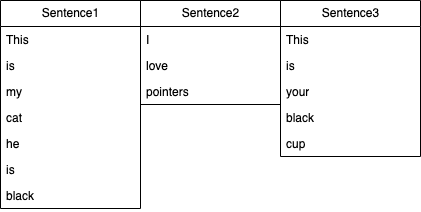
\includegraphics[width=0.6\textwidth]{example2.png}  % Replace 'example.png' with your image file name and specify the width
\end{figure}

%\acknowledgement{Ak niekomu chcete poďakovať\ldots}


% týmto sa generuje zoznam literatúry z obsahu súboru literatura.bib podľa toho, na čo sa v článku odkazujete
\bibliography{literatura}
\bibliographystyle{plain} % prípadne alpha, abbrv alebo hociktorý iný
\end{document}
